\documentclass[border=10pt]{standalone}
\usepackage{tikz}
\usetikzlibrary{shapes.geometric, arrows.meta, positioning}
\usepackage{fontawesome}

\definecolor{miamired}{RGB}{200,16,46} % Define miamired color

\begin{document}

\begin{tikzpicture}[node distance=2cm, auto]

% Styles
\tikzstyle{central} = [circle, draw, align=center, fill=miamired, text=white, font=\bfseries\large, minimum size = 4cm]
\tikzstyle{outer} = [circle, draw=miamired, align=center, text=black, minimum size =4cm, font=\bfseries\small]

% Central node
\node (cia) [central] {CIA};

% Surrounding nodes
\node (conf) [outer, above left=of cia, xshift=-1cm] {\faLock\\ Confidentiality};
\node (integ) [outer, above right=of cia, xshift=1cm] {\faCheckCircle\\ Integrity};
\node (avail) [outer, below=of cia] {\faCloud\\ Availability};

% Arrows
\draw [-Latex, miamired] (cia) -- (conf);
\draw [-Latex, miamired] (cia) -- (integ);
\draw [-Latex, miamired] (cia) -- (avail);

\end{tikzpicture}

\end{document}
